%%=============================================================================
%% H3 - Ontwerpprincipes van ZFS
%%=============================================================================

\chapter{Ontwerpprincipes \& architectuur van ZFS}
\label{ch:h3}

In dit hoofdstuk worden enkele principes besproken waarop de ontwikkelaars zich hebben gebaseerd bij het ontwerp en de ontwikkeling van ZFS. Tevens wordt de architectuur van ZFS globaal beschreven, om zo de ontwerpbeslissingen van de ontwikkelaars wat meer toe te lichten.

\section{Ontwerpprincipes}

De principes die aan de basis van ZFS liggen vloeiden meestal voort uit de problemen die de ontwikkelaars zelf ervaarden bij het gebruik van andere bestandssystemen.

\subsection{Eenvoud van beheer \& Storage Pools}

Volgens \textcite{ZFSBonwick} kan en moet het aanmaken en beheren van bestandssystemen een stuk makkelijker gemaakt worden. Hierbij speelt automatisatie van verschillende taken een belangrijke rol. Ook moet het mogelijk zijn om beheerderstaken (zoals bestandssystemen aanmaken en verwijderen) uit te voeren zonder de werking van het gehele systeem te ondermijnen \autocite{ZFSBonwick}. 

Een niet onbelangrijke feature hierbij zijn storage pools. Storage pools hebben als doel om opslagruimte zoveel mogelijk los te koppelen van de fysieke schijven: alle schijven bevinden zich in een pool van disks. Uit deze pool kunnen bestandssystemen worden aangemaakt, zonder rekening te moeten houden met de limitaties van bv. partities. Tevens kunnen bestandssystemen op een flexibele manier gebruik maken van deze pooled storage door automatisch in te krimpen en uit te breiden wanneer nodig \autocite{ZFSBonwick}. 

\begin{figure}
        \centering
        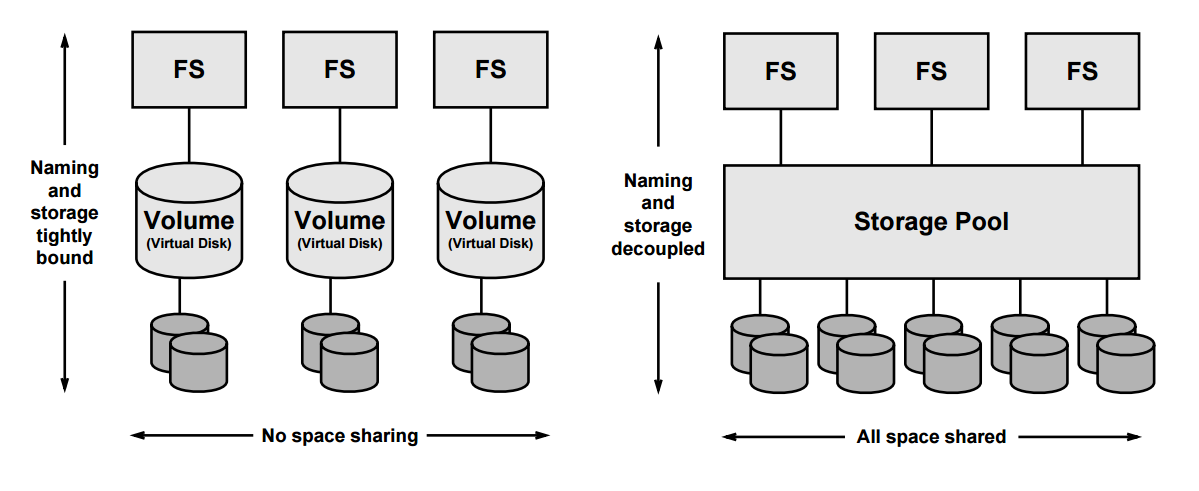
\includegraphics[width=0.8\textwidth]{h3-pools-vs-vols}
        \caption{Illustratie van ZFS pooled storage (rechts) t.o.v.volume-based storage (links) \autocite{ZFSBonwick}}
        \label{fig:bonwick_pools_illustratie}
\end{figure}
  
\subsection{Consistentie \& Integriteit}

Eén van de taken van een bestandssysteem is om ervoor te zorgen dat het in een consistente toestand blijft, i.e. het moet mogelijk zijn om van inconsistente toestanden te herstellen d.m.v. bijvoorbeeld een journal of door een filesystem check te draaien \autocite{OSThreePiecesRemzi2015}. Een nadeel aan deze technieken volgens \textcite{ZFSBonwick} is dat deze niet makkelijk zijn om te implementeren, omdat bijvoorbeeld in het geval van journaling filesystems een roll back of roll forward moet worden uitgevoerd. Hierbij moet ook nog de volgorde van de bewerkingen in acht worden genomen \autocite{OSThreePiecesRemzi2015}. 

De oplossing volgens \textcite{ZFSBonwick} is om het bestandssysteem te allen tijde consistent te houden; er mag m.a.w. geen enkel moment zijn waarop het systeem in een inconsistente toestand kan terecht komen. Dit wordt verwezenlijkt door de Copy-On-Write eigenschappen van ZFS, waardoor bewerkingen atomair gebeuren \autocite{Li2009}. 

Een ander aspect waar ZFS een antwoord op tracht te vinden, is het voorkomen en minimaliseren van datacorruptie. Volgens \textcite{ZFSBonwick} is het niet verstandig om volledig te vertrouwen op hardware, omdat er steeds een kans is dat deze bugs bevat. Dit kan leiden tot \textit{silent data corruption}: dit is een fenomeen waarbij de schijf corrupte datablokken niet kan detecteren \autocite{OSThreePiecesRemzi2015}. Om deze reden bevat ZFS een uitgebreid checksumming-mechanisme dat werkt op blokniveau.
In Hoofdstuk \ref{ch:h4} wordt er dieper ingegaan op deze technieken.
% Indien men ZFS zou voorstellen als een boomstructuur, dan bevatten de \textit{parent blocks} steeds de checksums van hun kinderen \autocite{ZFSBonwick}. Bij het uitlezen en wegschrijven van een blok data wordt de checksum berekend en gecontroleerd met de (eventueel) reeds bestaande checksum. Indien deze overeenkomen, dan wordt het datablok doorgegeven. Indien deze niet overeenkomen, dan tracht ZFS het corrupte blok te repareren. Echter moet er wel opgemerkt worden dat er voor automatische foutcorrectie (goede) kopieën van de corrupte blokken moeten beschikbaar zijn \autocite{Li2009}.

\subsection{Ingebouwde volumebeheerder}

Indien bijvoorbeeld LVM (Logical Volume Manager) wordt gebruikt op een Linux-systeem voor het aanmaken van volumes, dan staan de volumes relatief "los"  van de bestandssystemen die worden aangemaakt op deze volumes: eerst maakt men volumes aan, nadien pas bestandssystemen \autocite{Lewis2006}. 

\textcite{ZFSBonwick} is van mening dat een volledige integratie van de volumebeheerder in het bestandssysteem een aantal interessante voordelen met zich meebrengt, zoals betere optimalisaties en betere consistentie, omdat de volume manager nu "weet" hoe de bestandssystemen in de storage pool(s) zijn opgebouwd.

\section{De architectuur van ZFS: een overzicht}

De architectuur van ZFS is opgebouwd uit een zestal componenten \autocite{Li2009}: de Storage Pool Allocator (SPA), de Data Management Unit (DMU), een ZFS POSIX Layer (ZPL), de ZFS Attribute Processor (ZAP), de ZFS Intent Log (ZIL) en ZFS Volume (ZVOL). Elk onderdeel biedt een bepaalde functionaliteit aan en levert diensten aan boven- en onderliggende lagen.

\subsection{Storage Pool Allocator (SPA)}

De taak van de SPA is hoofdzakelijk om datablokken van verschillende apparaten in één pool te verzamelen; de functionaliteit van de SPA komt m.a.w. in grote mate overeen met die van een volume manager. Het grote verschil tussen een volume manager en de SPA is dat de SPA louter een \textit{interface} is voor virtuele datablokken; dit in tegenstelling tot een volume manager, dat volumes doorgeeft aan het besturingssysteem \autocite{ZFSBonwick}. 

De Storage Pool Allocator biedt een interface aan tot \textbf{data virtual addresses (DVA's)}: dit zijn de adressen van de virtuele datablocks die zich in een storage pool bevinden. De datablokken die zich fysiek op een schijf bevinden worden dus niet rechtstreeks aangesproken; alle communicatie van bovenliggende lagen gericht tot de fysieke disks moet eerst via de SPA. Hierdoor worden de ontwerpprincipes van \textit{'Eenvoud van beheer'} en \textit{'Storage Pools'} gerealiseerd: schijven kunnen dynamisch worden toegevoegd zonder de werking van de rest van het systeem te ondermijnen. Ook kan de systeembeheerder op een flexibele manier bestandssystemen aanmaken, zonder rekenschap te moeten geven aan de onderliggende fysieke structuur \autocite{ZFSBonwick}.

Deze eigenschappen zjin te danken aan VDEV's (Virtual Devices). Dit zijn a.h.w. de bouwstenen van storage pools \autocite{Lucas2015}. Deze worden in Hoofdstuk \ref{ch:h5} wat meer toegelicht.

\subsection{Data Management Unit (DMU)}

De Data Management Unit is de laag boven de SPA en is a.h.w. de 'lijm' tussen de nogal \textit{low-level} (virtuele) datablokken en de bovenliggende lagen. Deze component vertaalt de blokken naar ZFS objecten; dit is nodig omdat ZFS alles voorstelt als objecten. Zo stelt een ZFS-object van het type \texttt{DMU\_OT\_ACL} een access control list voor \autocite{Microsystems2006}. Objecten behoren steeds tot een bepaalde naamruimte (\textit{namespace}) of dataset; dit verhoogt de flexibiliteit m.b.t. het beheer van bestandssystemen aanzienlijk. Zo wordt een bestandssysteem binnen ZFS voorgesteld door objecten uit een bepaalde dataset. Aangezien objecten van elkaar gescheiden zijn door private namespaces, leven bestandssystemen (die uit een reeks van ZFS-objecten bestaan) ook naast en onafhankelijk van elkaar. Dit maakt taken zoals aanmaken en verwijderen van filesystems een stuk makkelijker voor zowel de gebruiker als de DMU \autocite{ZFSBonwick}.   

Daarnaast staat de DMU ook garant voor de consistentie van alle data. Om deze reden worden transacties binnen ZFS geïmplementeerd door de Data Management Unit als COW-transacties (Copy-On-Write). Hierbij wordt gebruik gemaakt van een 'alles of niets'-aanpak: ofwel is de transactie gelukt, ofwel is de transactie mislukt en moeten er back-upblokken worden aangewend \autocite{ZFSBonwick}.

\begin{figure}
        \centering
        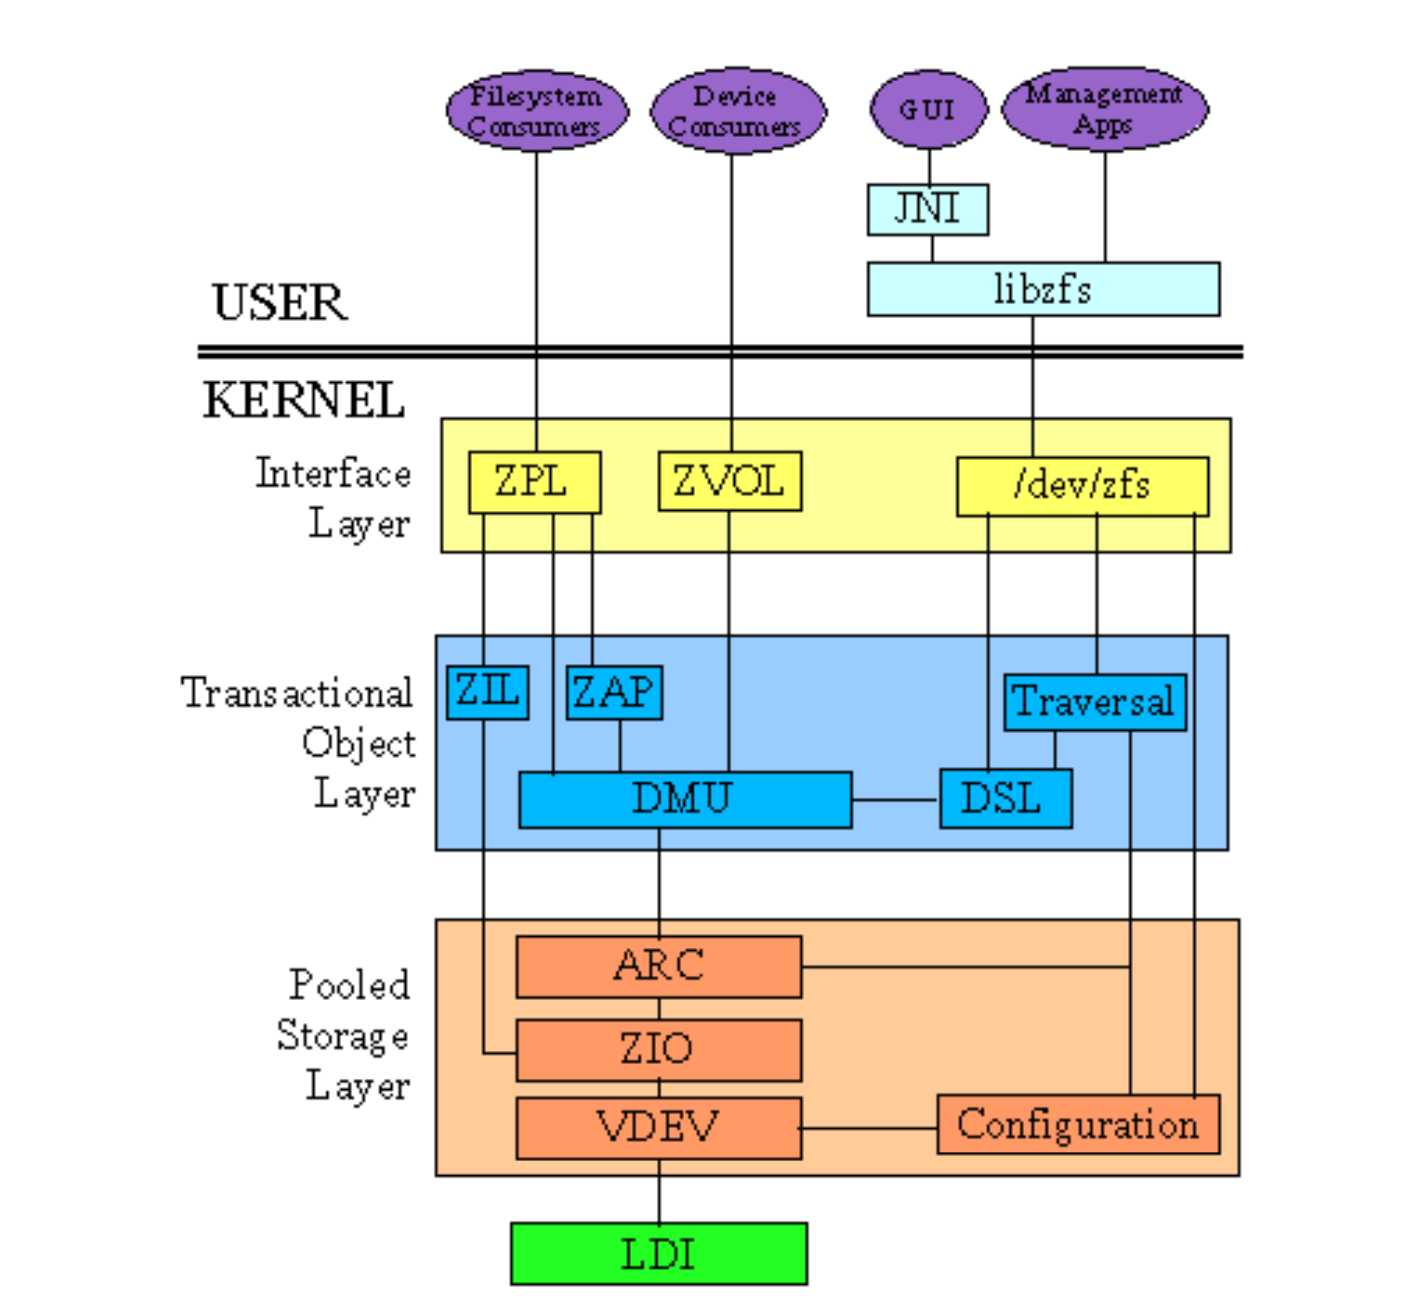
\includegraphics[width=0.7\textwidth]{h3-zfs_overview}
        \caption{Een overzicht van de verschillende componenten van ZFS \autocite{KendiOnbekend}}
        \label{fig:kendi_zfs_overview}
\end{figure}

\subsection{ZFS POSIX Layer (ZPL)}

Deze laag vertaalt objecten komende van de Data Management Unit naar met POSIX compatibele bestandssystemen \autocite{ZFSBonwick}. POSIX (acroniem voor Portable Operating System Interface) is een reeks van standaarden waaraan ontwikkelaars zich moeten houden indien ze willen dat hun programma's \textit{portable} (overdraagbaar) zijn. Dit betekent dat het weinig tot geen moeite zou moeten kosten voor een ontwikkelaar om een programma draaiende te krijgen op bv. verschillende UNIX-systemen \autocite{IEEE2016}. Solaris en macOS zijn voorbeelden van 'POSIX-compliant' besturingssystemen \autocite{GroupOnbekend}.

Voor het uitvoeren van bewerkingen maakt de ZPL gebruik van de onderliggende Data Management Unit. Het aanmaken van een bestandssysteem gebeurt bijvoorbeeld door de ZFS POSIX Layer: de ZPL maakt enkele DMU-objecten met metadata e.d. aan en maakt gebruik van het transactiemodel van de DMU om deze objecten weg te schrijven. Dankzij deze aanpak verlopen deze bewerkingen ook atomair \autocite{ZFSBonwick}. 

\subsection{ZFS Attribute Processor (ZAP)}

De ZFS Attribute Processor is een component die samenwerkt met de DMU-laag. De ZAP manipuleert ZAP-objecten: dit zijn speciale DMU-objecten die metadata over allerhande dingen bijhouden in de vorm van key-value pairs. Deze informatie handelt over verschillende andere objecten, zoals datasets en filesystem objects. Voor een grote hoeveelheid attributen (en dus informatie) wordt er gebruikgemaakt van zgn. fatzaps; indien de hoeveelheid informatie nogal gering is, dan kiest ZFS voor microzaps \autocite{Microsystems2006}.

\subsection{ZFS Intent Log (ZIL)}

Deze component houdt logbestanden bij van alle transacties voor het geval dat het bestandssysteem toch in een inconsistente toestand zou terecht komen, bijvoorbeeld bij een stroompanne. Op deze manier kunnen transacties worden gereplayed indien consistentie van uiterst belang is. Deze records worden bijgehouden in het RAM-geheugen tot ze worden gepersisteerd door een DMU-transactie of door een \texttt{fsync} \autocite{ZFSBonwick}. 

\subsection{ZFS Volume (ZVOL)}

ZFS Volumes of ZVOL's zijn objecten die binnen ZFS worden voorgesteld als een koppel van een property object en een dataobject. Deze logische volumes worden dan aan het OS doorgegeven als ordinaire UNIX block devices en kunnen ook op deze manier benaderd worden \autocite{Microsystems2006}.
